\documentclass[14pt,a4paper]{article}

\usepackage{fullpage}
\usepackage[utf8]{inputenc}
\usepackage{lmodern}
\usepackage{amsmath}
\usepackage{amssymb}
\usepackage{amsfonts}
\usepackage{pgfplots}
\usepackage{tikz}
\usepackage{pgf}

\begin{document}
% start
\qquad
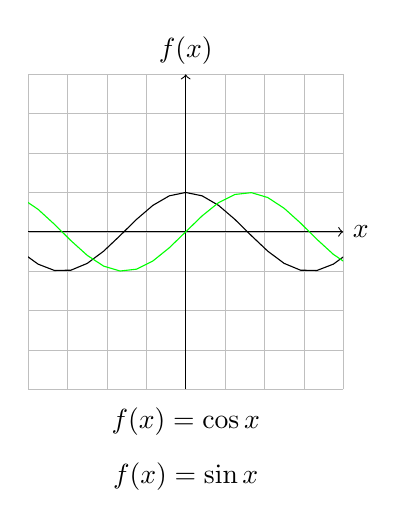
\begin{tikzpicture}[scale=0.5]
\draw[very thin,color=lightgray] (-4,-4) grid (4,4);
    \draw[->] (-4,0) -- (4,0) node[right] {$x$};
    \draw[->] (0,-4) -- (0,4) node[above] {$f(x)$};
    \draw node[below=60pt] {$f(x) = \cos x$};
    \draw node[below=80pt] {$f(x) =  \sin x$}; 
    \clip (-4,-4) rectangle (4,4);
    \draw[color=black] plot (\x,{cos(\x r)});
    \draw[color=green]   plot (\x,{sin(\x r)}); 
\end{tikzpicture}
\qquad
\vspace{\baselineskip}
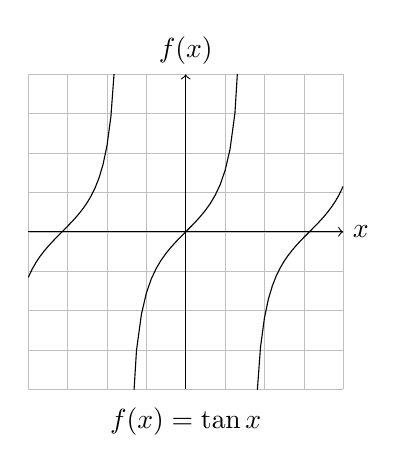
\begin{tikzpicture}[scale=0.5]
\draw[very thin, color=lightgray] (-4,-4) grid (4,4);
	\draw[->] (-4,0) -- (4,0) node[right] {$x$};
    \draw[->] (0,-4) -- (0,4) node[above] {$f(x)$};
    \draw node[below=60pt] {$f(x) = \tan x$};
    \clip (-4,-4) rectangle (4,4);
    \draw[color=black,domain=-1.5:1.5] plot (\x,{tan(\x r)});
    \draw[color=black,domain=-4:-1.6] plot (\x,{tan(\x r)});
    \draw[color=black,domain=1.6:4] plot (\x,{tan(\x r)});
\end{tikzpicture}
\qquad
\vspace{\baselineskip}
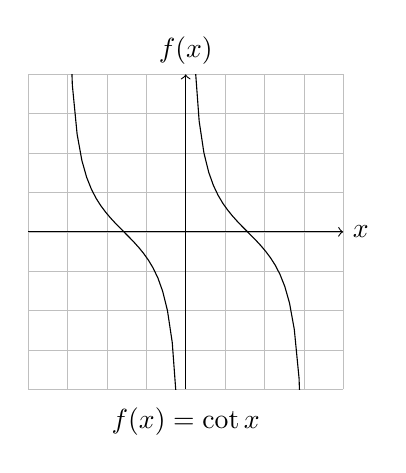
\begin{tikzpicture}[scale=0.5]
\draw[very thin, color=lightgray] (-4,-4) grid (4,4);
	\draw[->] (-4,0) -- (4,0) node [right] {$x$};
	\draw[->] (0,-4) -- (0,4) node [above] {$f(x)$};
	\draw node[below=60pt] {$f(x) = \cot x$};
	\clip (-4,-4) rectangle (4,4);
	\draw [color=black,domain=-3:-0.1]		plot (\x, {cot(\x r)});
	\draw [color=black,domain=0.1:3]	plot (\x, {cot(\x r)});
\end{tikzpicture}
\qquad
\vspace{\baselineskip}
$
\cos x=0$ für $x=(2k+1) \frac{\pi}{2}, k \in \mathbb{Z}$ \\ $
\sin x=0$ für $x=k \pi, k\in \mathbb{Z}
$ \\\\
\textit{Symmetrien: } \\
$
\cos(-x) = \cos(x) $ \\ $ 
\sin(-x) = -\sin(x) $ \\\\ 
Periode $ 2\pi 
\begin{cases} 
\cos(x+2 \pi) = \cos(x) \\
\sin(x+2 \pi) = \sin(x) 
\end{cases} $ \\ 
Periode $ \pi  
\begin{cases} 
\tan(x+\pi) = \tan x \\
\cot(x+\pi) = \cot x 
\end{cases} $
\\\\\\
\underline{Additionstheoreme}\\
$
\sin(x+y) = \sin x \cos y + \cos x \sin y $ \\ $
\cos(x+y) = \cos x \cos y - \sin x \sin y $ \\ 
speziell $ x=y $ \\ $
\sin(2x) = 3 \sin x \cos x $ \\ $
\cos(2x) = \cos^2 x - \sin^2 x $ \\ $ 
\tan(x+y) = \frac{\tan x + \tan y}{1-\tan x \tan y} $ \\\\ denn \[
\tan(x+y) = \frac{\sin(x+y)}{\cos(x+y)} = \frac{\sin x \cos y + \cos x \sin y}{\cos x \cos y - \sin x \sin y} * \frac{\frac{1}{(\cos x \cos y)}}{\frac{1}{(\cos x \cos y)}} 
= \frac{\frac{\sin x}{\cos x}+ \frac{\sin y}{\cos y}}{1- \frac{\sin x \sin y}{\cos x \cos y}} \] \\\\
\underline{Differentration} \\ $
\cos 'x = -\sin x $ \\ $
\sin 'x = \cos x $ \\ $
\tan 'x = 1 + \tan^2 x $ \\ $
\cot 'x = -(1+\cot^2 x) $ \\

% stop
\end{document}


